%Set up the document class.
\documentclass[11pt]{article}

%Include packages.
\usepackage[]{authblk}
\usepackage{pdflscape}
\usepackage{lipsum}
\usepackage{natbib}
\usepackage{float}
\usepackage{import}
\usepackage{enumitem}
\usepackage{etoolbox}
\usepackage[super]{nth}
\usepackage{hyperref}
\usepackage[ampersand]{easylist}
\usepackage{adjustbox}
\usepackage[toc,page]{appendix}
\usepackage{graphicx}
\graphicspath{{img/}}

%Commands
\newcommand\tab[1][1cm]{\hspace*{#1}}
\renewcommand{\labelenumii}{\Roman{enumii}}

\begin{document}

%The title page must be on it's own page.
%Create the title, affiliation section, and date.

%Add the logo.
\begin{figure}[t]
	
\includegraphics[scale=0.75]{northumbria_logo.jpg}
	\centering
\end{figure}	
\title{Project Idea}
\author{Group Name (TBD)}
\affil{Module: KV6002 - Team Project \& Professionalism\\~\\Northumbria University Newcastle}
\date{\today}
\maketitle

\newpage

\section*{Group Members}
\begin{table}[H]
	\centering
		\begin{tabular}{|l|l|}
			\hline
			\textbf{Student} & \textbf{Programme} \phantom{Computer Science with Games Development} \\ \hline
			Andrew Alford & Computer Science with Games Development              \\ \hline
			Alexandru-Daniel Pascal &  Computer Science with Games Development             \\ \hline
			Carl Pendleton &  Computer Science with Games Development             \\ \hline
			Alex Trench &  Computer Science             \\ \hline
			Haoming Yuan &  Computer Science with Games Development             \\ \hline
		\end{tabular}
\end{table}

\section*{Project Idea}
\subsection*{Summarised}
Develop a top-down shooter wave-based survival video game using Unreal Engine.
\subsection*{Developed}
This is a group project in which the five group members will each have their own individual subsystem to complete. Once completed, all these subsystems will be
combined into the final game. Collectively the group will be developing a top-down
shooter video game in which the player has to survive waves of enemy zombies. 
Many aspects of game developement such as level design, UI, XP \& progression will be included in the project. A fully functioning, playable, and bug-free game will
be produced by the end of the project. The final product will also be demonstrated
after production is finished.

\section*{Subsystems}
\subsection*{Enviroment \& Level Design}
\subsection*{Weapons}
\subsection*{Menus, UI \& Loading/Saving}
\subsection*{Levelling \& Progression}
\subsection*{Characters \& AI}

\section*{Project Client}
N/A

\section*{Project Stakeholders}
The target market - the players (needs to be elaborated on).

\section*{Existing Systems}
We are taking inspiration from many existing top-down ``twin-stick" shooters such as the examples detailed below. Tags for existing systens include:
\begin{itemize}
	\item Action
	\item Shooter
	\item Survival 
	\item Third Person
	\item Top-Down Shooter
	\item Twin Stick Shooter
\end{itemize}
\subsection*{Call of Duty: Dead-Ops Arcade}
\begin{figure}[H]
	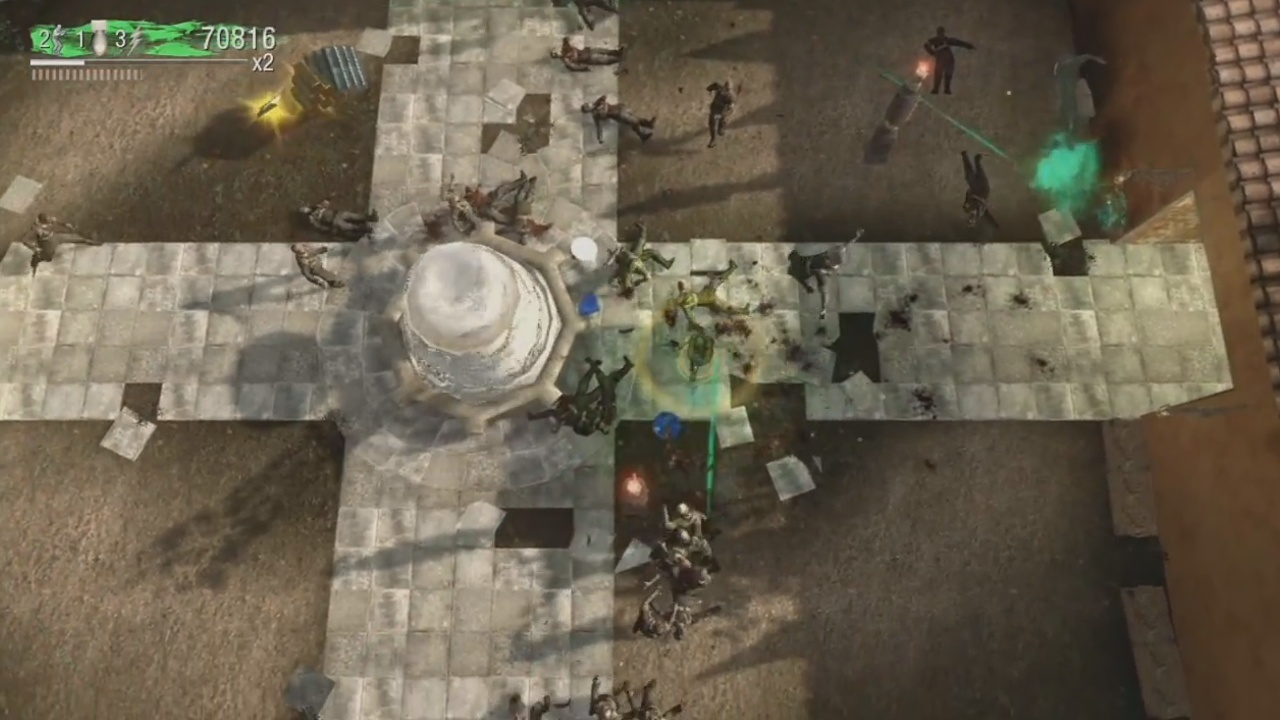
\includegraphics[scale=0.25]{call_of_duty_dead_ops_arcade.jpg}
	\centering
\end{figure}
\subsection*{Dead Island Epidemic}
\begin{figure}[H]
	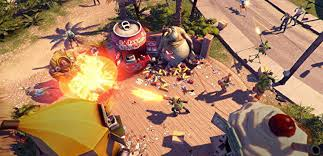
\includegraphics[scale=1]{dead_island.jpg}
	\centering
\end{figure}
\subsection*{Halo: Spartan Strike}
\begin{figure}[H]
	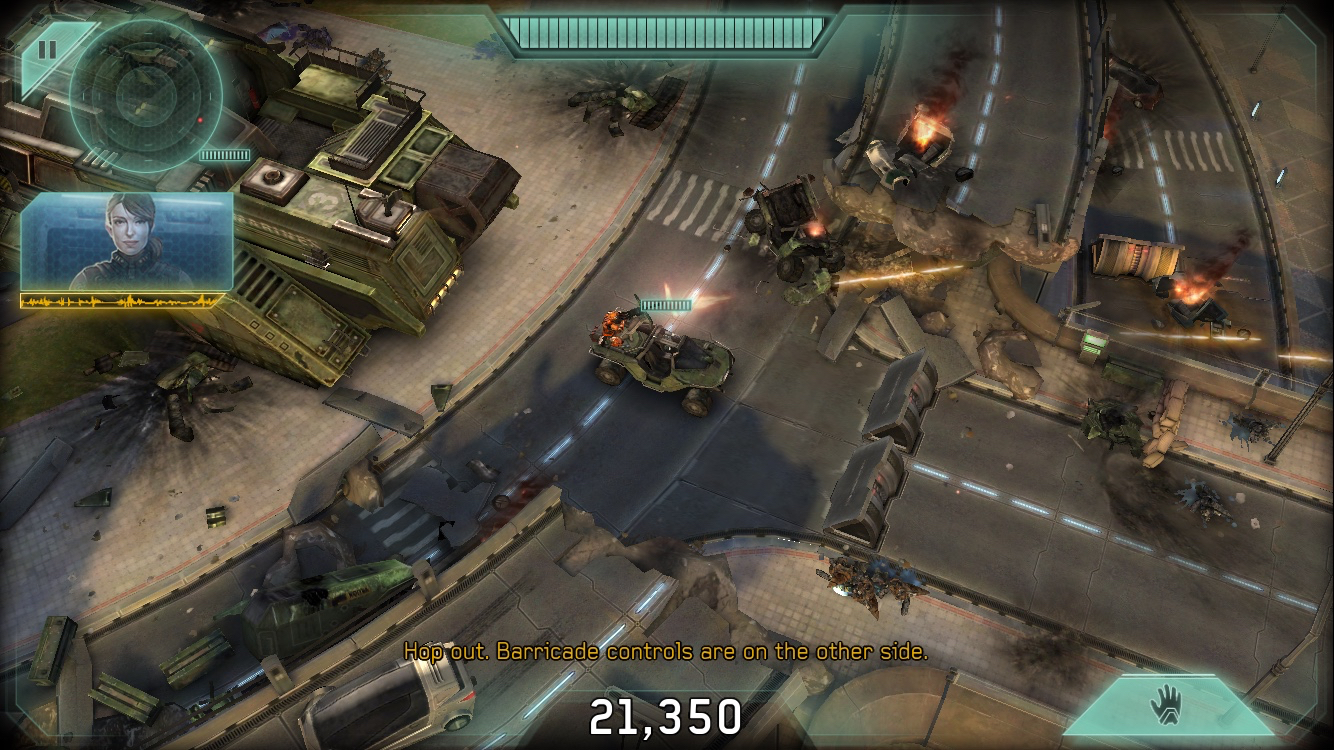
\includegraphics[scale=0.25]{halo_spartan_strike.jpg}
	\centering
\end{figure}
\subsection*{Warhammer 40,000: Kill Team}
\begin{figure}[H]
	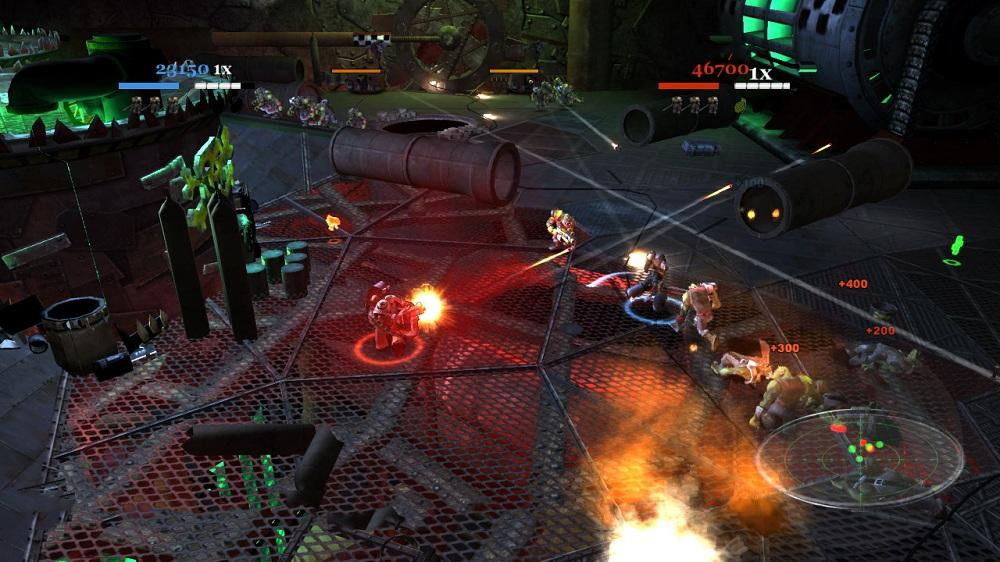
\includegraphics[scale=0.5]{warhammer.png}
	\centering
\end{figure}

\section*{Research}
Each team member will conduct research into their own subsection. Research
will include areas such as making an element of the game fun to play, designing
specific elements of the game, and implementing specific elements of the game.

\begin{table}[H]
\centering
\begin{tabular}{|l|l|}
\hline
\textbf{Project Idea} & \textbf{Date \& Time:} \phantom{This text will be invisible} \\ \hline
\textbf{Student} & \textbf{Signature}     \\ \hline
Andrew Alford           &               \\ \hline
Alexandru-Daniel Pascal &               \\ \hline
Carl Pendleton          &               \\ \hline
Alex Trench             &               \\ \hline
Haoming Yuan            &               \\ \hline
\end{tabular}
\end{table}



\end{document}